\chapter{Performance experiments}
Using a machine with a Ryzen 5 3600 CPU @ 3.7GHz and 32GB DDR4 @ 3200MHz memory we conduct several experiments with different inputs and settings, the results are shown in Tables \ref{tab:iterator-performance} through \ref{tab:pruning-performance-big}. 

For source graph-target graph pairs without a present vertex disjoint subgraph homeomorphism we consistently use the G(n, M) Erdős–Rényi random graph model.

Since vertex disjoint subgraph homeomorphisms are rare in random graphs, we construct source graph-target graph pairs with a present vertex disjoint subgraph homeomorphism by generating a random source graph and injecting vertices and edges to obtain a target graph. First we add vertices: with a 50\% probability we intersect a random existing edge with each new vertex and with 50\% probability we add it outside the existing graph. Then we add edges: while the vertices added outside the source graph have less-than-average degree we add uniformly sampled edges that include them; afterwards we add uniformly sampled random edges.


\begin{figure}
\centering
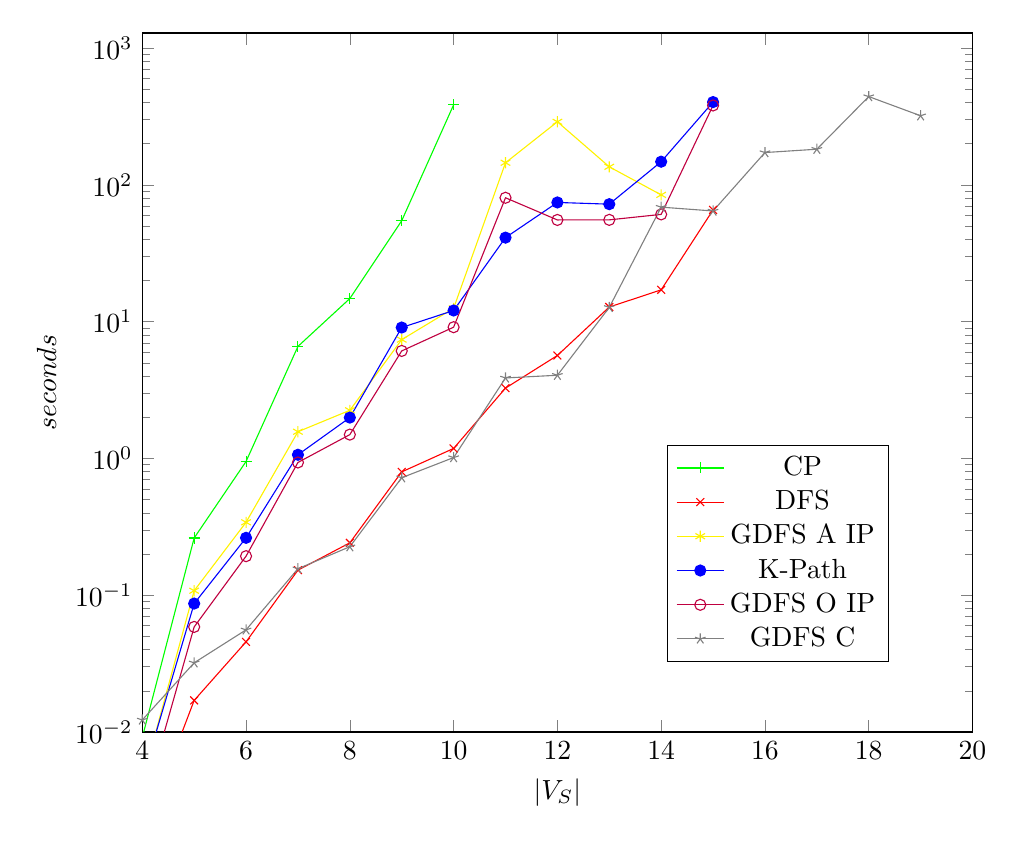
\begin{tikzpicture}
    \begin{axis}[
        xlabel=$|V_S|$,
        ylabel=$seconds$,
        ymin=0.01,
        ymode=log,
        xmin=4,
        xmax=20,
        legend style={at={(0.9,0.1)},anchor=south east},
        width=\textwidth,
    ]
    \addplot[
        mark=+,
        green,
    ] plot coordinates {
        (4,0.009108628025032595) 
        (5,0.2620836802188065) 
        (6,0.9503740113943355)
        (7,6.596783503767442) 
        (8,14.764050718975609) 
        (9,54.765670739272736)
        (10,385.16296629500005) 
};
    \addlegendentry{CP}
    
    
    
    \addplot[
        mark=x,
        red,
    ] plot coordinates {
        (4,0.001716029672925713)
        (5,0.01702360071809101) 
        (6,0.04561513035914958) 
        (7,0.15251165322667018) 
        (8,0.24155461744973755) 
        (9,0.797513732268617) 
        (10,1.1835030509211046) 
        (11,3.2680702187065216)
        (12,5.661746851933962) 
        (13,12.798846733085105)
        (14,17.096358927307694)
        (15,65.64831186045454)
};
    \addlegendentry{DFS}
    
    
    
    \addplot[
        mark=asterisk,
        yellow,
    ] plot coordinates {
        (4,0.0043272421728668435) 
        (5,0.1078318674295203) 
        (6,0.3413335015273159)
        (7,1.5682172603423914)
        (8,2.249343766891791) 
        (9,7.395351140134146)
        (10,12.526694290867926)
        (11,145.27286338419998) 
        (12,289.503897899)
        (13,135.6942000877143) 
        (14,84.56603693766665)
};
    \addlegendentry{GDFS A IP}
    
    
    \addplot[
        mark=*,
        blue,
    ] plot coordinates {
        (4,0.004513287361457468) 
        (5,0.08689765890565003)
        (6,0.26278218619322824)
        (7,1.0640096504880734) 
        (8,1.9899295945868851)
        (9,9.064827074119401)
        (10,12.07097279138)
        (11,41.171574928875)
        (12,74.45223459277778)
        (13,72.3320726255)
        (14,147.87316945775) 
        (15,403.442499958)
};
    \addlegendentry{K-Path}
    
    \addplot[
        mark=o,
        purple,
    ] plot coordinates {
        (4,0.0027085184446120963) 
        (5,0.05864821291835853) 
        (6,0.19300624213070725) 
        (7,0.9348330173258064)
        (8,1.4939211758271604)
        (9,6.113139861699029)
        (10,9.11535311513433) 
        (11,80.54225475566666)
        (12,55.450854962)
        (13,55.5386134715)
        (14,60.892068884249994) 
        (15,381.159786211)
};
    \addlegendentry{GDFS O IP}
    
    
    \addplot[
        mark=star,
        gray,
    ] plot coordinates {
        (4,0.012242439615384614) 
        (5,0.032056864899625934) 
        (6,0.05582594232351259) 
        (7,0.15618683271269063) 
        (8,0.22630326749716662)
        (9,0.7229805422695548)
        (10,1.0152932454602368)
        (11,3.8780944653607596)
        (12,4.058766762371621)
        (13,12.724517174693878)
        (14,68.79296791008333)
        (15,64.49375942241666)
        (16,172.4802085922)
        (17,182.4329892165)
        (18,442.59586222949997)
        (19,320.441386005)
};
    \addlegendentry{GDFS C}
    \end{axis}
    \end{tikzpicture}
    \caption{A comparison of the speed of path iterators on directed graphs. The time taken is measured of exploring the entire search tree without pruning or contraction and ``refuse longer paths" enabled. The source graph has average degree $3.0$ and the random target graph has $50\%$ more vertices and average degree $4.0$.}
\end{figure}

\begin{table}[ht]
\centering
\begin{tabular}{|l|l|l|l|l|l|l|}
\hline
\textbf{Path iteration} &
  \textbf{Its/success} &
  \textbf{Time/iteration} &
  \textbf{time/success} &
  \textbf{stdev} &
  \textbf{time/fail} &
  \textbf{stdev} \\ \hline
K-Path        &  &  &  &  &  &  \\ \hline
DFS           &  &  &  &  &  &  \\ \hline
Greedy DFS    &  &  &  &  &  &  \\ \hline
Control point &  &  &  &  &  &  \\ \hline
\end{tabular}
\caption{Performance of different path iteration methods on random source graphs of size $|V|\in \{8..12\}$ with edge density 3.0 and random target graphs of size $|V|\in \{15..20\}$ with edge density 4.0. ``refuse unnecessarily long paths" and contraction are enabled and parallel all-different pruning is used.}
\label{tab:iterator-performance}
\end{table}




\begin{table}[ht]
\centering
\begin{tabular}{|l|l|l|l|l|l|l|}
\hline
\textbf{Path iteration} &
  \textbf{Its/success} &
  \textbf{Time/iteration} &
  \textbf{time/success} &
  \textbf{stdev} &
  \textbf{time/fail} &
  \textbf{stdev} \\ \hline
K-Path        &  &  &  &  &  &  \\ \hline
DFS           &  &  &  &  &  &  \\ \hline
Greedy DFS    &  &  &  &  &  &  \\ \hline
Control point &  &  &  &  &  &  \\ \hline
\end{tabular}
\caption{Performance of different path iteration methods on random source graphs of size $|V|\in \{1..5\}$ with edge density 3.0 and a square of four ECP5 logic tiles as target graph. ``refuse unnecessarily long paths" and contraction are enabled and parallel all-different pruning is used.}
\label{tab:iterator-performance}
\end{table}

\begin{table}[ht]
\centering
\begin{tabular}{|l|l|l|l|l|l|}
\hline
\textbf{Source graph size} & \textbf{Target graph size} & \textbf{K-Path} & \textbf{DFS} & \textbf{Greedy DFS} & \textbf{CP} \\ \hline
$|V|=5$, $|E|=10$          & $|V|=8$, $|E|=15$          & -30.0\%                     & +10.0\%          &  -20.0\%                      & -17.0\%               \\ \hline
&&&&&\\\hline
&&&&&\\\hline
&&&&&\\\hline
&&&&&\\\hline
&&&&&\\\hline
&&&&&\\\hline
                           & single ECP5 tile         &                           &                &                        &                \\ \hline
                                                      & square of ECP5 tiles         &                           &                &                        &                \\ \hline
\end{tabular}
\caption{The performance benefit (seconds) of the `refuse unnecessarily long paths' setting on random source graphs and random target graphs.}
\label{tab:refuselongerpaths-performance}
\end{table}



\begin{table}[ht]
\centering
\begin{tabular}{|l|l|l|l|l|l|}
\hline
\textbf{Source graph size} & \textbf{Target graph size} & \textbf{K-Path} & \textbf{DFS} & \textbf{Greedy DFS} & \textbf{CP} \\ \hline
$|V|=5$, $|E|=10$          & $|V|=8$, $|E|=15$          & -30.0\%                     & +10.0\%          &  -20.0\%                      & -17.0\%               \\ \hline
&&&&&\\\hline
&&&&&\\\hline
&&&&&\\\hline
&&&&&\\\hline
&&&&&\\\hline
&&&&&\\\hline
                           & single ECP5 tile         &                           &                &                        &                \\ \hline
                                                      & square of ECP5 tiles         &                           &                &                        &                \\ \hline
\end{tabular}
\caption{The performance benefit (seconds) of contraction on random source graphs and random target graphs.}
\label{tab:contraction-performance}
\end{table}




% Please add the following required packages to your document preamble:
% \usepackage{multirow}
\begin{table}[]
\begin{tabular}{|l|l|l|l|l|}
\hline
\textbf{Pruning strategy}      & \textbf{Filtering}               & \textbf{Application} & \textbf{Effect (+)} & \textbf{Effect (-)} \\ \hline
None                           &                                  &                      & +0.0\%              & +0.0\%              \\ \hline
\multirow{12}{*}{Zero domain}  & \multirow{3}{*}{Label/degree}    & Serial               &                     &                     \\ \cline{3-5} 
                               &                                  & Cached               &                     &                     \\ \cline{3-5} 
                               &                                  & Parallel             &                     &                     \\ \cline{2-5} 
                               & \multirow{3}{*}{Free neighbours} & Serial               &                     &                     \\ \cline{3-5} 
                               &                                  & Cached               &                     &                     \\ \cline{3-5} 
                               &                                  & Parallel             &                     &                     \\ \cline{2-5} 
                               & \multirow{3}{*}{M-reachability}  & Serial               &                     &                     \\ \cline{3-5} 
                               &                                  & Cached               &                     &                     \\ \cline{3-5} 
                               &                                  & Parallel             &                     &                     \\ \cline{2-5} 
                               & \multirow{3}{*}{N-reachability}  & Serial               &                     &                     \\ \cline{3-5} 
                               &                                  & Cached               &                     &                     \\ \cline{3-5} 
                               &                                  & Parallel             &                     &                     \\ \hline
\multirow{12}{*}{AllDifferent} & \multirow{3}{*}{Label/degree}    & Serial               &                     &                     \\ \cline{3-5} 
                               &                                  & Cached               &                     &                     \\ \cline{3-5} 
                               &                                  & Parallel             &                     &                     \\ \cline{2-5} 
                               & \multirow{3}{*}{Free neighbours} & Serial               &                     &                     \\ \cline{3-5} 
                               &                                  & Cached               &                     &                     \\ \cline{3-5} 
                               &                                  & Parallel             &                     &                     \\ \cline{2-5} 
                               & \multirow{3}{*}{M-reachability}  & Serial               &                     &                     \\ \cline{3-5} 
                               &                                  & Cached               &                     &                     \\ \cline{3-5} 
                               &                                  & Parallel             &                     &                     \\ \cline{2-5} 
                               & \multirow{3}{*}{N-reachability}  & Serial               &                     &                     \\ \cline{3-5} 
                               &                                  & Cached               &                     &                     \\ \cline{3-5} 
                               &                                  & Parallel             &                     &                     \\ \hline
\end{tabular}
\caption{The performance effect (seconds) of different pruning methods with- and without Connectivity check (CC) and neighbour check (NC) on random source graphs of size $|V|\in \{8..12\}$ with edge density 3.0 and a square of four ECP5 times as target graph. Effect (+) denotes cases with some homeomorphism and Effect (-) denotes cases without a homemorphism.}
\label{tab:pruning-performance-small}
\end{table}



% Please add the following required packages to your document preamble:
% \usepackage{multirow}
\begin{table}[]
\begin{tabular}{|l|l|l|l|l|}
\hline
\textbf{Pruning strategy}      & \textbf{Filtering}               & \textbf{Application} & \textbf{Effect (+)} & \textbf{Effect (-)} \\ \hline
None                           &                                  &                      & +0.0\%              & +0.0\%              \\ \hline
\multirow{12}{*}{Zero domain}  & \multirow{3}{*}{Label/degree}    & Serial               &                     &                     \\ \cline{3-5} 
                               &                                  & Cached               &                     &                     \\ \cline{3-5} 
                               &                                  & Parallel             &                     &                     \\ \cline{2-5} 
                               & \multirow{3}{*}{Free neighbours} & Serial               &                     &                     \\ \cline{3-5} 
                               &                                  & Cached               &                     &                     \\ \cline{3-5} 
                               &                                  & Parallel             &                     &                     \\ \cline{2-5} 
                               & \multirow{3}{*}{M-reachability}  & Serial               &                     &                     \\ \cline{3-5} 
                               &                                  & Cached               &                     &                     \\ \cline{3-5} 
                               &                                  & Parallel             &                     &                     \\ \cline{2-5} 
                               & \multirow{3}{*}{N-reachability}  & Serial               &                     &                     \\ \cline{3-5} 
                               &                                  & Cached               &                     &                     \\ \cline{3-5} 
                               &                                  & Parallel             &                     &                     \\ \hline
\multirow{12}{*}{AllDifferent} & \multirow{3}{*}{Label/degree}    & Serial               &                     &                     \\ \cline{3-5} 
                               &                                  & Cached               &                     &                     \\ \cline{3-5} 
                               &                                  & Parallel             &                     &                     \\ \cline{2-5} 
                               & \multirow{3}{*}{Free neighbours} & Serial               &                     &                     \\ \cline{3-5} 
                               &                                  & Cached               &                     &                     \\ \cline{3-5} 
                               &                                  & Parallel             &                     &                     \\ \cline{2-5} 
                               & \multirow{3}{*}{M-reachability}  & Serial               &                     &                     \\ \cline{3-5} 
                               &                                  & Cached               &                     &                     \\ \cline{3-5} 
                               &                                  & Parallel             &                     &                     \\ \cline{2-5} 
                               & \multirow{3}{*}{N-reachability}  & Serial               &                     &                     \\ \cline{3-5} 
                               &                                  & Cached               &                     &                     \\ \cline{3-5} 
                               &                                  & Parallel             &                     &                     \\ \hline
\end{tabular}
\caption{The performance effect (seconds) of different pruning methods with- and without Connectivity check (CC) and neighbour check (NC) on random source graphs of size $|V|\in \{8..12\}$ with edge density 3.0 and a square of four ECP5 times as target graph. Effect (+) denotes cases with some homeomorphism and Effect (-) denotes cases without a homemorphism.}
\label{tab:pruning-performance-big}
\end{table}
